\renewcommand*{\arraystretch}{1.1}

\label{sec:bi-read-24}
\noindent\begin{tabularx}{\queryCardWidth}{|>{\queryPropertyCell}c|X|}
	\hline
	query & BI / 24 \\ \hline
%
	title & Messages by Topic and Continent \\ \hline
%
    pattern & \hfill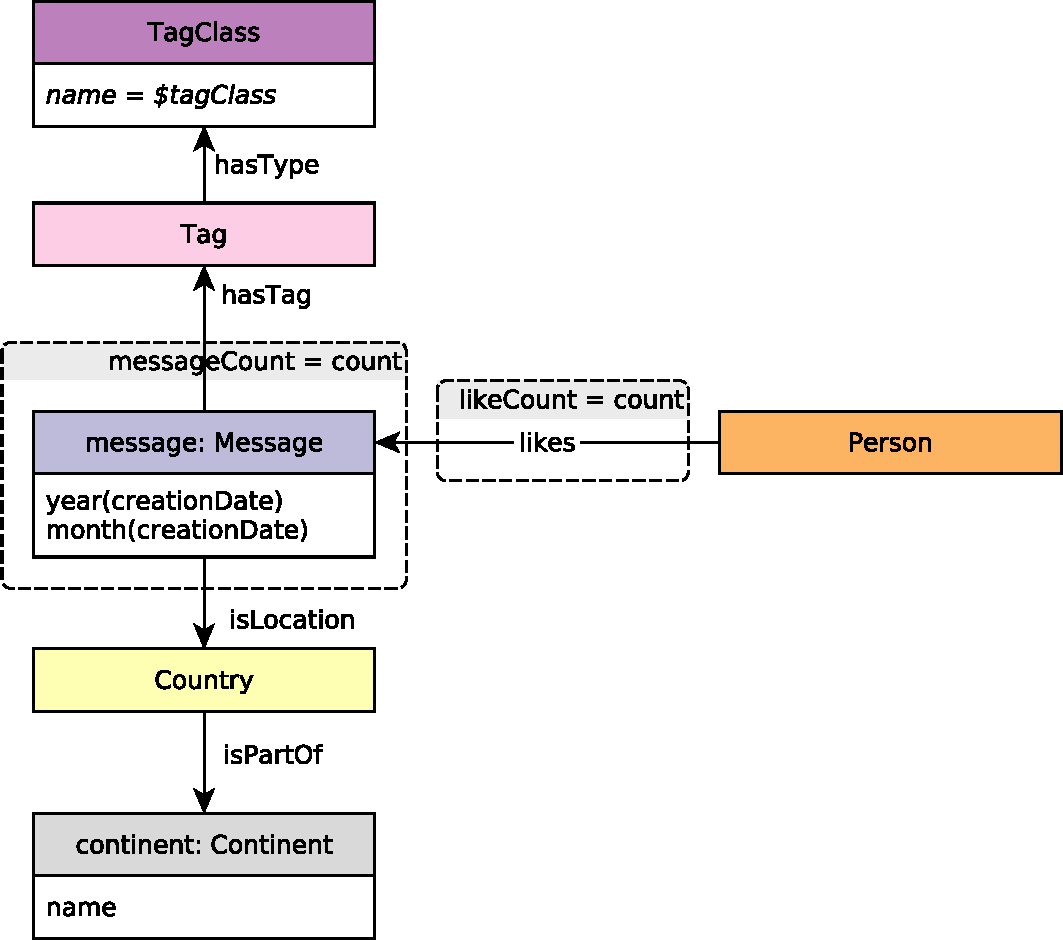
\includegraphics[scale=\patternscale,margin=0cm .2cm]{patterns/bi-read-24}\hfill\vadjust{} \\ \hline
%
	desc. & Find all Messages tagged with a Tag from the given TagClass
(non-transitive).

Count all messages and their likes grouped by continent, year, and
month. (TODO - do we group the Messages or the Persons who liked the
Messages by continent? I think the former one - szarnyasg)
 \\ \hline
%
	
        group by &
        \multicolumn{1}{>{\raggedright}X|}{
            \varNameText year, 
            \varNameText month, 
            \varNameText continent.name
            } \\ \hline
	
%
	params &
	\innerCardVSpace{\begin{tabularx}{\attributeCardWidth}{|>{\paramNumberCell}c|>{\varNameCell}M|>{\typeCell}m{\typeWidth}|Y|} \hline
	\cellcolor{parameter} \color{white} \footnotesize $\mathsf{1}$ &tagClass& String &  \\ \hline
	\end{tabularx}}\innerCardVSpace \\ \hline
%
	
        result &
        \innerCardVSpace{\begin{tabularx}{\attributeCardWidth}{|>{\resultNumberCell}c|>{\varNameCell}M|>{\typeCell}m{\typeWidth}|>{\resultOriginCell}c|Y|} \hline
        $\mathsf{1}$ & messageCount & 32-bit Integer &A&
                 \\ \hline
        $\mathsf{2}$ & likeCount & 32-bit Integer &A&
                 \\ \hline
        $\mathsf{3}$ & year & 32-bit Integer &C&
                year of the Message's creationDate \\ \hline
        $\mathsf{4}$ & month & 32-bit Integer &C&
                month of the Message's creationDate \\ \hline
        $\mathsf{5}$ & continent.name & String &R&
                 \\ \hline
        \end{tabularx}}\innerCardVSpace \\ \hline
	
%
	sort        &
        \innerCardVSpace{\begin{tabular}{|>{\sortNumberCell}c|>{\varNameCell}l|>{\directionCell}c|} \hline
        $\mathsf{1}$ & year & $\asc$ \\ \hline
        $\mathsf{2}$ & month & $\asc$ \\ \hline
        $\mathsf{3}$ & continent.name & $\desc$ \\ \hline
        \end{tabular}}\innerCardVSpace \\ \hline
	%
	limit & 100 \\ \hline
	%
	CPs &
	\multicolumn{1}{>{\raggedright}l|}{
	    \chokePoint{1.6}, 
	    \chokePoint{2.1}, 
	    \chokePoint{2.3}, 
	    \chokePoint{2.4}, 
	    \chokePoint{3.2}, 
	    \chokePoint{4.3}
	    } \\ \hline
	%
    %
\end{tabularx}
\queryCardVSpace